\documentclass[unicode,11pt,a4paper,oneside,numbers=endperiod,openany]{scrartcl}
\usepackage{amsmath} 
\usepackage{amsfonts}
\usepackage{graphicx}
\usepackage{enumitem} 
\usepackage{longtable}
\usepackage{array}
\usepackage{xcolor}
\usepackage{booktabs}
\usepackage{multirow}
\usepackage{geometry}
\usepackage{listings}
\lstdefinestyle{mystyle}{
    basicstyle=\ttfamily\small,
    keywordstyle=\color{blue},
    commentstyle=\color{green},
    stringstyle=\color{red},
    numbers=left,
    numberstyle=\tiny,
    stepnumber=1,
    frame=single,
    breaklines=true,
    captionpos=b,
    tabsize=2
}

\lstdefinelanguage{MyC++}{
    language=C++,
    morekeywords={std, vector, string},
}

\lstdefinelanguage{MyPython}{
    language=Python,
    morekeywords={self},
}

\lstdefinelanguage{MyBatch}{
    morekeywords={echo, pause, set},
    sensitive=false, 
    morecomment=[l]{REM}, 
    morestring=[b]",
}

\lstdefinelanguage{MyBash}{
    basicstyle=\ttfamily,
    breaklines=true,
    frame=single,
    keywordstyle=\color{blue},
    commentstyle=\color{gray},
    showstringspaces=false
}
\usepackage{ifthen}
\usepackage[utf8]{inputenc}
\usepackage{graphics}
\usepackage{graphicx}
\usepackage{hyperref}

\pagestyle{plain}
\voffset -5mm
\oddsidemargin  0mm
\evensidemargin -11mm
\marginparwidth 2cm
\marginparsep 0pt
\topmargin 0mm
\headheight 0pt
\headsep 0pt
\topskip 0pt        
\textheight 255mm
\textwidth 165mm

\newcommand{\duedate} {}
\newcommand{\setduedate}[1]{%
\renewcommand\duedate {See iCorsi for due date}}
\newcommand\isassignment {false}
\newcommand{\setassignment}{\renewcommand\isassignment {true}}
\newcommand{\ifassignment}[1]{\ifthenelse{\boolean{\isassignment}}{#1}{}}
\newcommand{\ifnotassignment}[1]{\ifthenelse{\boolean{\isassignment}}{}{#1}}

\newcommand{\assignmentpolicy}{
\begin{table}[h]
\begin{center}
\scalebox{0.8} {%
\begin{tabular}{|p{0.02cm}p{16cm}|}
\hline
&\\
\multicolumn{2}{|c|}{\Large\textbf{HPC Lab ---  Submission Instructions}}\\
\multicolumn{2}{|c|}{\large\textbf{(Please, notice that following instructions are mandatory: }}\\
\multicolumn{2}{|c|}{\large\textbf{submissions that don't comply with, won't be considered)}}\\
&\\
\textbullet & Assignments must be submitted to \href{https://www.icorsi.ch}{iCorsi} (i.e. in electronic format).\\
\textbullet & Provide both executable package and sources (e.g. C/C++ files, Matlab). 
If you are using libraries, please add them in the file. Sources must be organized in directories called:\\
\multicolumn{2}{|c|}{\textit{Project\_number\_lastname\_firstname}}\\
& and  the  file must be called:\\
\multicolumn{2}{|c|}{\textit{project\_number\_lastname\_firstname.zip}}\\
\multicolumn{2}{|c|}{\textit{project\_number\_lastname\_firstname.pdf}}\\
\textbullet &  The TAs will grade your project by reviewing your project write-up, and looking at the implementation 
                 you attempted, and benchmarking your code's performance.\\

\textbullet & You are allowed to discuss all questions with anyone you like; however: (i) your submission must list anyone you discussed problems with and (ii) you must write up your submission independently.\\
\hline
\end{tabular}
}
\end{center}
\end{table}
}
\newcommand{\punkte}[1]{\hspace{1ex}\emph{\mdseries\hfill(#1~\ifcase#1{Points}\or{Points}\else{Points}\fi)}}


\newcommand\serieheader[6]{
\thispagestyle{empty}%
\begin{flushleft}

\includegraphics[width=0.4\textwidth]{usi_inf.png}
\end{flushleft}
  \noindent%
  {\large\ignorespaces{\textbf{#1}}\hspace{\fill}\ignorespaces{ \textbf{#2}}}\\ \\%
  {\large\ignorespaces #3 \hspace{\fill}\ignorespaces #4}\\
  \noindent%
  \bigskip
  \hrule\par\bigskip\noindent%
  \bigskip {\ignorespaces {\Large{\textbf{#5}}}
  \hspace{\fill}\ignorespaces \large \ifthenelse{\boolean{\isassignment}}{\duedate}{#6}}
  \hrule\par\bigskip\noindent%  \linebreak
 }

\makeatletter
\def\enumerateMod{\ifnum \@enumdepth >3 \@toodeep\else
      \advance\@enumdepth \@ne
      \edef\@enumctr{enum\romannumeral\the\@enumdepth}\list
      {\csname label\@enumctr\endcsname}{\usecounter
        {\@enumctr}%%%? the following differs from "enumerate"
	\topsep0pt%
	\partopsep0pt%
	\itemsep0pt%
	\def\makelabel##1{\hss\llap{##1}}}\fi}
\let\endenumerateMod =\endlist
\makeatother




\usepackage{textcomp}





\begin{document}


\setassignment

\serieheader{High-Performance Computing Lab}{Institute of Computing}{Student: Zitian Wang}{Discussed with: Ning Ding; Xiaorui Wang}{Solution for Project 3}{}
\newline

\assignmentpolicy
This project will introduce you a parallel space solution of a nonlinear PDE using OpenMP.

\section{Task: Implementing the linear algebra functions and the stencil operators}
\subsection{Implement the functions }
\begin{lstlisting}[language=MyC++, style=mystyle, caption={HPC Norm Calculation}]
double hpc_norm2(Field const& x, const int N) {
    double result = 0;

    // TODO
    if(N == 0){
        return 0.0;
    }
    for(int i = 0; i < N; i++){
        result += x[i] * x[i];
    }

    return sqrt(result);
}
\end{lstlisting}
\begin{lstlisting}[language=MyC++, style=mystyle, caption={HPC Fill Function}]
void hpc_fill(Field& x, const double value, const int N) {
    // TODO
    for(int i = 0; i < N; i++){
        x[i] = value;
    }
}
\end{lstlisting}
\begin{lstlisting}[language=MyC++, style=mystyle, caption={HPC AXPY Function}]
void hpc_axpy(Field& y, const double alpha, Field const& x, const int N) {
    // TODO
    for (int i = 0; i < N; i++){
        y[i] += alpha * x[i]; 
    }
}
\end{lstlisting}
\begin{lstlisting}[language=MyC++, style=mystyle, caption={HPC Add Scaled Difference Function}]
void hpc_add_scaled_diff(Field& y, Field const& x, const double alpha,
                          Field const& l, Field const& r, const int N) {
    // TODO
    for (int i = 0; i < N; i++){
        y[i] = x[i] + alpha * (l[i] - r[i]);
    }
}
\end{lstlisting}
\begin{lstlisting}[language=MyC++, style=mystyle, caption={HPC Scaled Difference Function}]
void hpc_scaled_diff(Field& y, const double alpha, Field const& l,
                      Field const& r, const int N) {
    // TODO
    for (int i = 0; i < N; i++){
        y[i] = alpha * (l[i] - r[i]);
    }
}
\end{lstlisting}
\begin{lstlisting}[language=MyC++, style=mystyle, caption={HPC Scale Function}]
void hpc_scale(Field& y, const double alpha, Field const& x, const int N) {
    // TODO
    for (int i = 0; i < N; i++){
        y[i] = alpha * x[i];
    }
}
\end{lstlisting}
\begin{lstlisting}[language=MyC++, style=mystyle, caption={HPC Linear Combination Function}]
void hpc_lcomb(Field& y, const double alpha, Field const& x, const double beta,
                Field const& z, const int N) {
    // TODO
    for (int i = 0; i < N; i++){
        y[i] = alpha * x[i] + beta * z[i];
    }
}
\end{lstlisting}
\begin{lstlisting}[language=MyC++, style=mystyle, caption={HPC Copy Function}]
void hpc_copy(Field& y, Field const& x, const int N) {
    // TODO
    for (int i = 0; i < N; i++){
        y[i] = x[i];
    }
}
\end{lstlisting}
\subsection{Implement the kernel}  
\begin{lstlisting}[language=MyC++, style=mystyle, caption={Interior Grid Points Calculation}]
// the interior grid points
for (int j = 1; j < jend; j++) {
    for (int i = 1; i < iend; i++) {
        // TODO
        // f(i,j) = ...
        f(i, j) = -(4.0 + alpha) * s_new(i, j)
              + s_new(i + 1, j) + s_new(i - 1, j)
              + s_new(i, j + 1) + s_new(i, j - 1)
              + alpha * s_old(i, j)
              + beta * s_new(i, j) * (1.0 - s_new(i, j));
    }
}
\end{lstlisting}
\subsection{Plot the solution}
\begin{lstlisting}[language=MyC++, style=mystyle, caption={Mini-Stencil Program Output}]
[wangzi@icsnode30 mini_app]$ ./main 128 100 0.005
=======================================================================
                      Welcome to mini-stencil!
version   :: C++ Serial
mesh      :: 128 * 128 dx = 0.00787402
time      :: 100 time steps from 0 .. 0.005
iteration :: CG 300, Newton 50, tolerance 1e-06
=======================================================================
-----------------------------------------------------------------------
simulation took 0.223021 seconds
1514 conjugate gradient iterations, at rate of 6788.61 iters/second
300 newton iterations
-----------------------------------------------------------------------
### 1, 128, 100, 1514, 300, 0.223021 ###
Goodbye!
\end{lstlisting}
\begin{figure}[h]
  \centering
  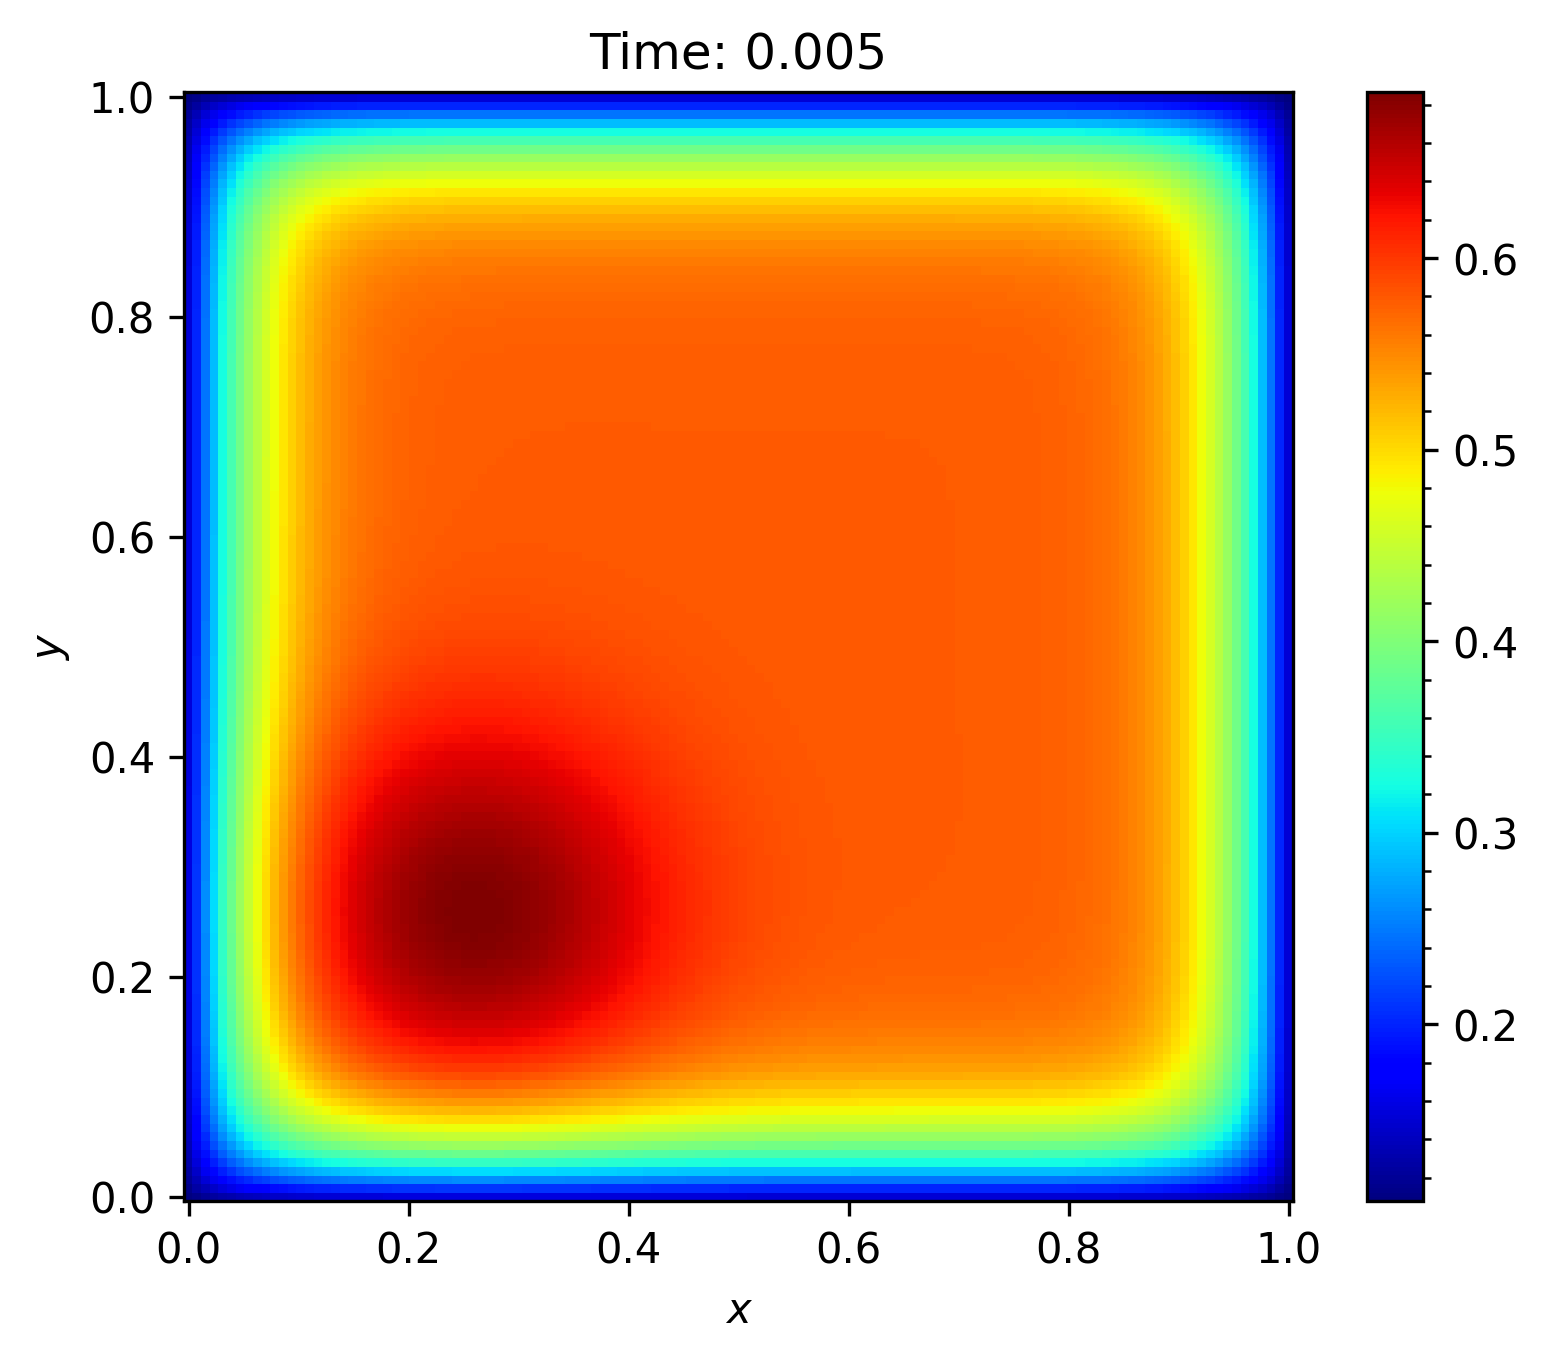
\includegraphics[width=0.25\textwidth]{pictures/output.png}
  \caption{The population concentration at time t = 0.005}
\end{figure}

\section{Task:  Adding OpenMP to the nonlinear PDE mini-app}
\subsection{Replace the welcome message}
\begin{lstlisting}[language=MyC++, style=mystyle, caption={Mini-Stencil Program Output with OpenMP}]
[wangzi@icsnode33 mini_app]$ ./main 128 100 0.005
==========================================================================
                      Welcome to mini-stencil!
version   :: C++ OpenMP
threads   :: 4
mesh      :: 128 * 128 dx = 0.00787402
time      :: 100 time steps from 0 .. 0.005
iteration :: CG 300, Newton 50, tolerance 1e-06
==========================================================================
--------------------------------------------------------------------------
simulation took 0.145261 seconds
1515 conjugate gradient iterations, at rate of 10429.5 iters/second
300 newton iterations
--------------------------------------------------------------------------
### 4, 128, 100, 1515, 300, 0.145261 ###
Goodbye!
\end{lstlisting}
\subsection{Linear algebra kernel}
To avoid conflict between different threads updating the same value at the same time, the parallel function for \texttt{hpc\_dot} and \texttt{hpc\_norm2 uses}:

\texttt{\# pragma omp parallel for reduction (+: result)}

Other functions use:

\texttt{\# pragma omp parallel for}.

\begin{lstlisting}[language=MyC++, style=mystyle, caption={HPC Dot Product Function with Parallelization}]
double hpc_dot(Field const& x, Field const& y, const int N) {
    double result = 0;
    #pragma omp parallel for reduction(+:result)
    for (int i = 0; i < N; i++) {
        result += x[i] * y[i];
    }

    return result;
}
\end{lstlisting}
\begin{lstlisting}[language=MyC++, style=mystyle, caption={HPC Norm Calculation Function with Parallelization}]
double hpc_norm2(Field const& x, const int N) {
    double result = 0;

    // TODO
    if(N == 0){
        return 0.0;
    }
    #pragma omp parallel for reduction(+:result)
    for(int i = 0; i < N; i++){
        result += x[i] * x[i];
    }

    return sqrt(result);
}
\end{lstlisting}
\begin{lstlisting}[language=MyC++, style=mystyle, caption={HPC Fill Function with Parallelization}]
void hpc_fill(Field& x, const double value, const int N) {
    // TODO
    #pragma omp parallel for
    for(int i = 0; i < N; i++){
        x[i] = value;
    }
}
\end{lstlisting}
\begin{lstlisting}[language=MyC++, style=mystyle, caption={HPC AXPY Function with Parallelization}]
void hpc_axpy(Field& y, const double alpha, Field const& x, const int N) {
    // TODO
    #pragma omp parallel for
    for (int i = 0; i < N; i++){
        y[i] += alpha * x[i]; 
    }
}
\end{lstlisting}
\begin{lstlisting}[language=MyC++, style=mystyle, caption={HPC Add Scaled Difference Function with Parallelization}]
void hpc_add_scaled_diff(Field& y, Field const& x, const double alpha,
                          Field const& l, Field const& r, const int N) {
    // TODO
    #pragma omp parallel for
    for (int i = 0; i < N; i++){
        y[i] = x[i] + alpha * (l[i] - r[i]);
    }
}
\end{lstlisting}
\begin{lstlisting}[language=MyC++, style=mystyle, caption={HPC Scaled Difference Function with Parallelization}]
void hpc_scaled_diff(Field& y, const double alpha, Field const& l,
                      Field const& r, const int N) {
    // TODO
    #pragma omp parallel for
    for (int i = 0; i < N; i++){
        y[i] = alpha * (l[i] - r[i]);
    }
}
\end{lstlisting}
\begin{lstlisting}[language=MyC++, style=mystyle, caption={HPC Scale Function with Parallelization}]
void hpc_scale(Field& y, const double alpha, Field const& x, const int N) {
    // TODO
    #pragma omp parallel for
    for (int i = 0; i < N; i++){
        y[i] = alpha * x[i];
    }
}
\end{lstlisting}
\begin{lstlisting}[language=MyC++, style=mystyle, caption={HPC Linear Combination Function with Parallelization}]
void hpc_lcomb(Field& y, const double alpha, Field const& x, const double beta,
                Field const& z, const int N) {
    // TODO
    #pragma omp parallel for
    for (int i = 0; i < N; i++){
        y[i] = alpha * x[i] + beta * z[i];
    }
}
\end{lstlisting}
\begin{lstlisting}[language=MyC++, style=mystyle, caption={HPC Copy Function with Parallelization}]
void hpc_copy(Field& y, Field const& x, const int N) {
    // TODO
    #pragma omp parallel for
    for (int i = 0; i < N; i++){
        y[i] = x[i];
    }
}
\end{lstlisting}
\subsection{The diffusion stencil}
For code with double loop, should use \texttt{\#pragma omp parallel for collapse(2)} to parallel.
\begin{lstlisting}[language=MyC++, style=mystyle, caption={Parallelized Interior Grid Points Calculation with Collapse}]
  // the interior grid points
  #pragma omp parallel for collapse(2)
  for (int j = 1; j < jend; j++) {
      for (int i = 1; i < iend; i++) {
          // TODO
          // f(i,j) = ...
          f(i, j) = -(4.0 + alpha) * s_new(i, j)
                + s_new(i + 1, j) + s_new(i - 1, j)
                + s_new(i, j + 1) + s_new(i, j - 1)
                + alpha * s_old(i, j)
                + beta * s_new(i, j) * (1.0 - s_new(i, j));
      }
  }
\end{lstlisting}
For code with independence loop, use \texttt{\#pragma omp parallel for} for parallel. The role of boundary loops is to impose these boundary conditions on the boundaries of the mesh so that the entire simulation conforms to the real physical boundaries.
\begin{lstlisting}[language=MyC++, style=mystyle, caption={Parallelized Boundary Calculation for East and West Boundaries}]
  // east boundary
  {
      int i = nx - 1;
      #pragma omp parallel for
      for (int j = 1; j < jend; j++) {
          f(i, j) = -(4.0 + alpha) * s_new(i, j)
                 + s_new(i - 1, j) + bndE[j]
                 + s_new(i, j - 1) + s_new(i, j + 1)
                 + alpha * s_old(i, j)
                 + beta * s_new(i, j) * (1.0 - s_new(i, j));
      }
  }

  // west boundary
  {
      int i = 0;
      #pragma omp parallel for
      for (int j = 1; j < jend; j++) {
          f(i, j) = -(4.0 + alpha) * s_new(i, j)
                 + bndW[j]      + s_new(i + 1, j)
                 + s_new(i, j - 1) + s_new(i, j + 1)
                 + alpha * s_old(i, j)
                 + beta * s_new(i, j) * (1.0 - s_new(i, j));
      }
  }
\end{lstlisting}
Since each corner point is a different, independent computation, use \texttt{\#pragma omp parallel sections} to compute each corner point separately in parallel.
\begin{lstlisting}[language=MyC++, style=mystyle, caption={Parallelized North and South Boundaries Calculation with Sections}]
  // north boundary (plus NE and NW corners)
  #pragma omp parallel sections
  {
      #pragma omp section
      {
          int j = nx - 1;
          int i = 0; // NW corner
          f(i, j) = -(4.0 + alpha) * s_new(i, j)
                 + bndW[j]      + s_new(i + 1, j)
                 + s_new(i, j - 1) + bndN[i]
                 + alpha * s_old(i, j)
                 + beta * s_new(i, j) * (1.0 - s_new(i, j));
      }

      #pragma omp section
      {
          int j = nx - 1;
          for (int i = 1; i < iend; i++) {
              f(i, j) = -(4.0 + alpha) * s_new(i, j)
                     + s_new(i - 1, j) + s_new(i + 1, j)
                     + s_new(i, j - 1) + bndN[i]
                     + alpha * s_old(i, j)
                     + beta * s_new(i, j) * (1.0 - s_new(i, j));
          }
      }

      #pragma omp section
      {
          int j = nx - 1;
          int i = nx - 1; // NE corner
          f(i, j) = -(4.0 + alpha) * s_new(i, j)
                 + s_new(i - 1, j) + bndE[j]
                 + s_new(i, j - 1) + bndN[i]
                 + alpha * s_old(i, j)
                 + beta * s_new(i, j) * (1.0 - s_new(i, j));
      }
  }

  // south boundary (plus SW and SE corners)
  #pragma omp parallel sections
  {
      #pragma omp section
      {
          int j = 0;
          int i = 0; // SW corner
          f(i, j) = -(4.0 + alpha) * s_new(i, j)
                 + bndW[j] + s_new(i + 1, j)
                 + bndS[i] + s_new(i, j + 1)
                 + alpha * s_old(i, j)
                 + beta * s_new(i, j) * (1.0 - s_new(i, j));
      }

      #pragma omp section
      {
          int j = 0;
          for (int i = 1; i < iend; i++) {
              f(i, j) = -(4.0 + alpha) * s_new(i, j)
                     + s_new(i - 1, j) + s_new(i + 1, j)
                     + bndS[i]      + s_new(i, j + 1)
                     + alpha * s_old(i, j)
                     + beta * s_new(i, j) * (1.0 - s_new(i, j));
          }
      }

      #pragma omp section
      {
          int j = 0;
          int i = nx - 1; // SE corner
          f(i, j) = -(4.0 + alpha) * s_new(i, j)
                 + s_new(i - 1, j) + bndE[j]
                 + bndS[i]      + s_new(i, j + 1)
                 + alpha * s_old(i, j)
                 + beta * s_new(i, j) * (1.0 - s_new(i, j));
      }
  }
\end{lstlisting}

\subsection{Bitwise Identical Results in OpenMP PDE Solvers}

In general, it is difficult to guarantee bitwise-identical results when using a threaded OpenMP PDE solver. The primary reason lies in the \textbf{non-associativity of floating-point arithmetic}:

\begin{equation}
    (a + b) + c \neq a + (b + c)
\end{equation}

In sequential execution, floating-point operations follow a fixed order, whereas in parallel execution, the order of operations can change depending on thread scheduling. When using OpenMP, the \texttt{reduction} clause creates local copies of the variable for each thread, leading to discrepancies in the order of summation. The final combination of these local results is non-deterministic, which can lead to small variations due to rounding.

Moreover, the use of \textbf{parallel reduction in OpenMP} makes achieving identical results particularly challenging:
\begin{itemize}
    \item \textbf{Thread Scheduling:} OpenMP schedules threads differently across runs, leading to variations in floating-point addition.
    \item \textbf{Hardware and Compiler Effects:} Different compilers, compiler options, and hardware architectures can produce different rounding behaviors.
\end{itemize}

In conclusion, it is generally not feasible to achieve bitwise-identical results across parallel runs of an OpenMP-based PDE solver due to floating-point arithmetic limitations. Ensuring strict ordering would require serial reduction, significantly reducing parallel efficiency, thus making it impractical for performance-critical applications.

\subsection{Strong scaling}
Strong scaling refers to the study of the performance improvement when increasing the number of threads while keeping the problem size constant. In our analysis, we considered different grid resolutions, specifically $64 \times 64$, $128 \times 128$, $256 \times 256$, $512 \times 512$, and $1024 \times 1024$. We ran the simulation using $N_{CPU} = 1, 2, 4, 8, 16$ threads and recorded the solution time for each configuration.

The figure below shows the relationship between the number of threads and the time to solution for different resolutions. Ideally, as the number of threads increases, the time to solution should decrease proportionally, demonstrating good scalability.

\begin{figure}[h]
    \centering
    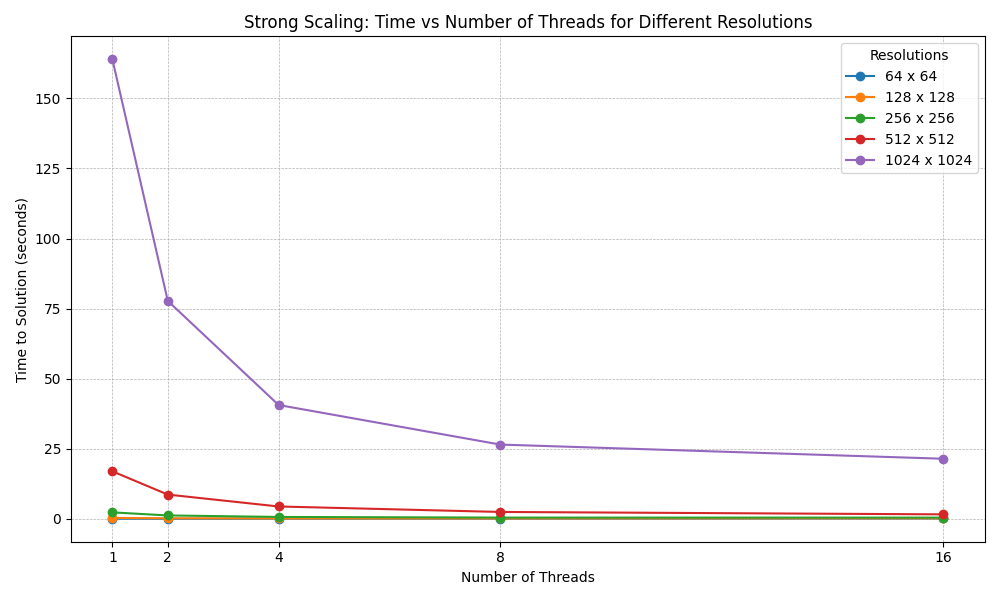
\includegraphics[width=0.8\textwidth]{pictures/strong_scaling_plot.png}
    \caption{Strong Scaling: Time vs Number of Threads for Different Resolutions. The plot shows how the time to solution decreases with the increasing number of threads, at various resolutions from $64 \times 64$ to $1024 \times 1024$.}
\end{figure}

The strong scaling results indicate that as the number of threads increases, the time to solution does decrease; however, the scaling efficiency diminishes beyond a certain point. For lower resolutions (e.g., $64 \times 64$), the overhead of managing multiple threads leads to suboptimal performance, particularly when more threads are used. This effect is less pronounced at higher resolutions (e.g., $1024 \times 1024$), where there is enough workload to justify the usage of additional threads.

Moreover, the diminishing returns observed as the number of threads increases can be attributed to the overheads associated with thread synchronization and the limited parallelism available in smaller problem sizes. This is consistent with Amdahl's Law, which states that the speedup of a parallel program is limited by the fraction of the code that cannot be parallelized.

The performance bottlenecks observed suggest that careful consideration must be given to the balance between problem size and the number of threads. For small problem sizes, increasing the number of threads beyond a certain point may yield little to no benefit and can even degrade performance due to increased communication overhead.
\subsection{Weak scaling}
Weak scaling refers to the study of performance as both the number of threads and the problem size increase proportionally, thereby maintaining a constant workload per thread. In this analysis, we explored different base resolutions ($64 \times 64$, $128 \times 128$, $256 \times 256$) and measured the time to solution using $N_{CPU} = 1, 2, 4, 8, 16$ threads, while proportionally increasing the problem size to maintain a constant load per thread.

The figure below presents the weak scaling results, showing the relationship between the number of threads and the time to solution while maintaining the workload per thread constant.

\begin{figure}[h]
    \centering
    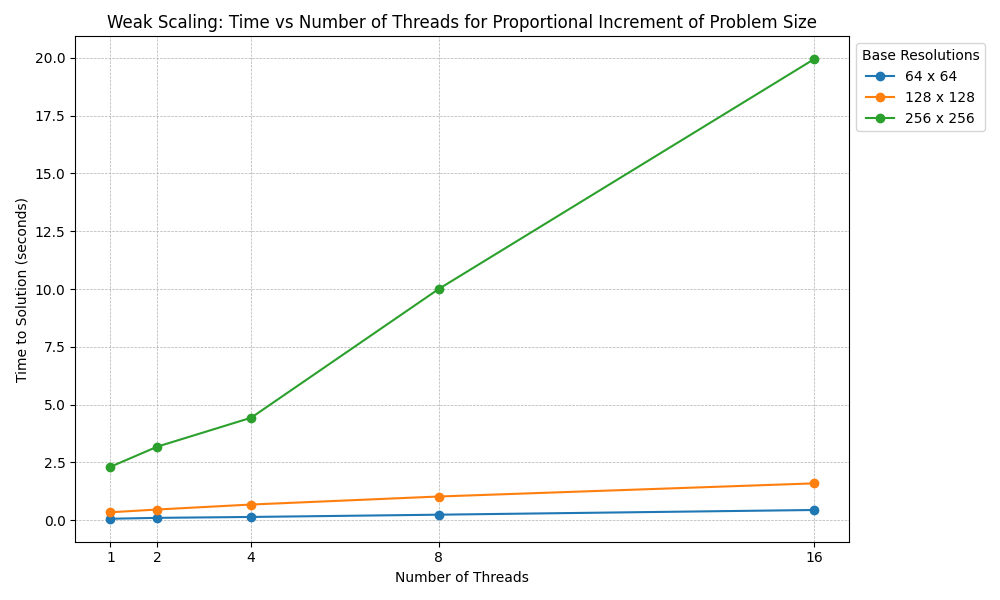
\includegraphics[width=0.8\textwidth]{pictures/weak_scaling_plot.png}
    \caption{Weak Scaling: Time vs Number of Threads for Proportional Increment of Problem Size. This plot illustrates the effect of increasing both the number of threads and problem size in a balanced manner to maintain constant workload per thread.}
    \label{fig:weak_scaling}
\end{figure}

The weak scaling results demonstrate that, as expected, the time to solution increases gradually with the number of threads and corresponding increase in problem size. Ideally, with perfect weak scaling, the time to solution would remain constant; however, the results reveal a slight increase, especially for larger thread counts.

This behavior can be attributed to several factors:
\begin{itemize}
    \item \textbf{Communication Overheads}: As the number of threads increases, the communication between threads also increases, leading to overhead that affects overall performance.
    \item \textbf{Memory Access Contention}: More threads can result in increased contention for memory access, leading to performance bottlenecks, particularly for larger resolutions.
    \item \textbf{Synchronization Costs}: Maintaining a consistent workload across multiple threads requires synchronization, which adds overhead as the number of threads increases.
\end{itemize}

Despite these challenges, the overall weak scaling performance indicates reasonable efficiency, especially for moderate numbers of threads. The gradual increase in runtime with more threads suggests that the solver is able to manage larger workloads effectively, though improvements in minimizing communication overhead could further enhance scalability.

In conclusion, the weak scaling analysis highlights the importance of balancing workload distribution with efficient communication and memory access strategies to achieve optimal performance as the problem size and thread count increase in parallel systems.

\end{document}
